\documentclass{beamer}

\mode<presentation>
{
  \usetheme{default}      
  \usecolortheme{beaver}
  \usefonttheme{professionalfonts}  
  \setbeamertemplate{navigation symbols}{}
  \setbeamertemplate{caption}[numbered]
  \setbeamertemplate{footline}[frame number]
} 
\usepackage{graphicx}
\usepackage{tikz}
\usepackage[english]{babel}
\usepackage[utf8x]{inputenc}
\usepackage{graphicx}
\usepackage{booktabs} % For formal tables
\usepackage{times}
\usepackage{textcomp}
\usepackage{amsmath}
\usepackage{graphicx}
\usepackage{multirow}
\usepackage{algorithmic}
\usepackage{algorithm}
\usepackage{ragged2e}
 \apptocmd{\frame}{}{\justifying}{} % Allow optional arguments after frame.0
\renewcommand{\raggedright}{\justifying}
%\newtheorem{mydef}{Definition}
\newtheorem{myteo}{Theorem}
\newtheorem{mycor}{Corollary}
\newtheorem{mylemma}{Lemma}
\renewcommand{\footnotesize}{\tiny}
%\renewcommand{\footnotesize}{\scriptsize}


\usepackage[style=verbose]{biblatex}
\bibliography{biblio}


\renewcommand{\raggedright}{\justifying}


\usepackage{tcolorbox}
\tcbuselibrary{theorems}

\newtcbtheorem[number within=section]{mytheo}{Theorem}%
{colback=green!5,colframe=red!35!gray,fonttitle=\bfseries}{th}


\newtcbtheorem[number within=section]{mydef}{Definition}%
{colback=green!5,colframe=red!35!gray,fonttitle=\bfseries}{th}

\title[Your Short Title]{Optimización Evolutiva Multi-objetivo}
\author{Dr. Carlos Segura González}
\institute{Centro de Investigación de Matemáticas}
%\date{November 07, 2019}

\begin{document}

\begin{frame}
  \titlepage
\end{frame}

%\begin{frame}{Outline}
%\begin{itemize}
%\item Introduction
%\item Maximum Likelihood Estimate
%\item Proposal
%\item MIX-SQP Algorithm
%\item Experimental Validation
%\item Conclusions
%\end{itemize}
%\end{frame}
\begin{frame}{Esquema General}
\frametitle{Esquema General}
\tableofcontents
\end{frame}


\section{Introducción y antecedentes}



\begin{frame}{Optimizadores estocásticos poblacionales}
    \begin{itemize}
    \scriptsize
    \justifying
        \item Una meta-heurística es un proceso maestro que de forma iterativa guía y modifica un conjunto de operaciones heurísticas con el fin de producir soluciones de calidad de forma eficiente \footcite{voss2012meta}.
        \item Las meta-heurísticas poblacionales consideran múltiples soluciones en cada iteración.
        \item Algunas meta-heurísticas poblacionales más populares son las siguientes:
        \begin{itemize}
        \scriptsize
            \item Algoritmos genéticos (GA).
            \item Programación genética (GP).
            \item Programación evolutiva (EP).
            \item Evolución diferencial (DE).
            \item Estrategia evolutiva (ES).
            \item Algoritmos de estimación de distribución (EDA).
            \item Optimización por enjambre de particulas (PSO).
            \item Algoritmos de optimización por colonias de hormigas (ACO).
        \end{itemize}{}
    \end{itemize}{}
\end{frame}{}


\begin{frame}{Optimizadores estocásticos poblacionales}

\begin{figure}[H]
\centering
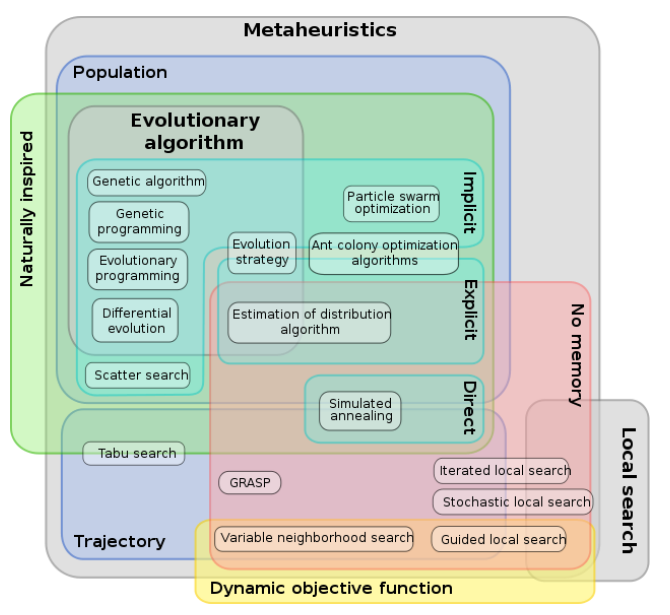
\includegraphics[width=0.6\textwidth]{clasificacion.png}
\caption{Clasificación de las meta-heurísticas más populares\footcite{beheshti2013review}.}
\label{fig:clasificacion}
\end{figure}
\end{frame}

\begin{frame}{Problemas de las meta-heurísticas poblacionales}
\begin{itemize}
    \item La mayoría de las meta-heurísticas poblacionales tienen problemas de convergencia, y no es fácil controlar la velocidad en que convergen.
   % \item Una de las fallas más típicas es la convergencia prematura.
%    \item La convergencia prematura es cuando los %miembros de la población son `atrapados' en ciertas regiones del espacio de búsqueda.
    \item Se dice que un algoritmo converge de forma prematura cuando mucho antes de alcanzar el criterio de paro, todas las soluciones están en una zona muy pequeña del espacio de búsqueda\footcite{Crepinsek:13}.
    
\begin{figure}[H]
\centering
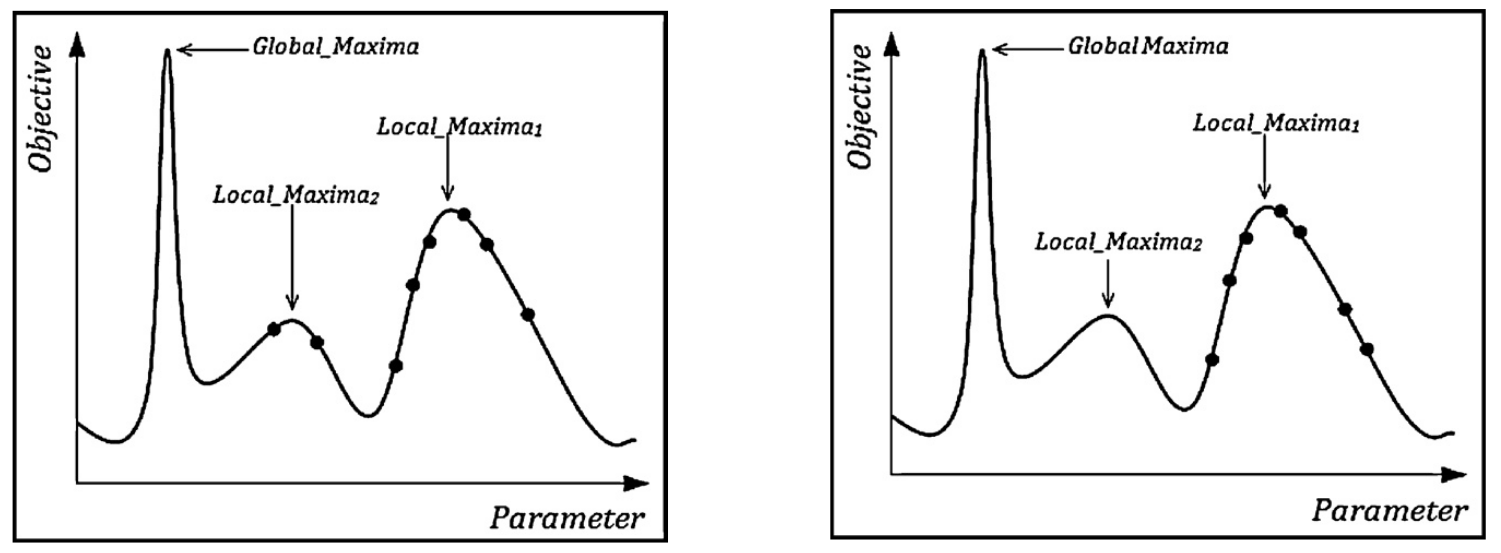
\includegraphics[width=0.7\textwidth]{landscape.png}
\caption{\scriptsize Escenarios de convergencia de una meta-heurística poblacional\footcite{alam2012diversity}.}
\label{fig:clasificacion}
\end{figure}
\end{itemize}
\end{frame}

\begin{frame}{Algoritmos Evolutivos (EAs)}
    \begin{itemize}
       \item Son un tipo de meta-heurísticas poblacionales.
        \item Son un enfoque ampliamente utilizado para resolver distintos tipos de problemas de optimización.
        
        \item Se han desarrollado diversas variantes que han sido aplicadas en múltiples campos, como en transporte, economía e ingeniería\footcite{dasgupta2013evolutionary}.
        
        \item Los EAs pueden ser aplicados en problemas de dominio continuo y/o de dominio discreto.
        
        \item Este tipo de algoritmos han sido exitosos principalmente en problemas del tipo NP-completo cuya solución exacta no es conocida.
    \end{itemize}{}
\end{frame}

\begin{frame}{Esquemas de los algoritmos evolutivos}
  \begin{algorithm}[H]
  \begin{scriptsize}
%\algsetup{linenosize=\tiny}
\caption{Evolutionary Algorithm} 
\begin{algorithmic}[1]
 	\STATE \textbf{Initialization}: Generate an initial population $P_0$ with $N$ individuals.
	\STATE \textbf{Evaluation}: Evaluate all individuals in the population.
	\STATE Assign $t=0$
	\WHILE{(not stopping criterion)}
	   \STATE \textbf{Mating selection}: Fill the mating pool performing selection on $P_t$.
	   \STATE \textbf{Variation}: Apply crossover and mutation operators to the mating pool to create an offspring population $Q_t$ with $N$ individuals.
		 \STATE \textbf{Evaluation}: Evaluate all individuals in $Q_t$.
	   \STATE \textbf{Survivor selection}: Generate $P_{t+1}$ by applying the replacement operator using $P_t$ and $Q_t$.
	   \STATE $t=t+1$
	\ENDWHILE
	\end{algorithmic}

\end{scriptsize}
\end{algorithm}
\end{frame}

\begin{frame}{Principios de diseño de un algoritmo poblacional}
\begin{itemize}
\justifying
    \item Como parte del diseño de una meta-heurística poblacional, para tratar adecuadamente la convergencia debería existir un balanceo entre \underline{exploración} e \underline{intensificación} del espacio de búsqueda \footcite{herrera1996adaptation}.
    \item La exploración del espacio de búsqueda evalúa regiones que no han sido muestreadas con el fin de detectar regiones promisorias.
    \item La intensificación realiza una búsqueda más profunda con el fin de encontrar soluciones de mayor calidad.
    
\end{itemize}
\begin{figure}
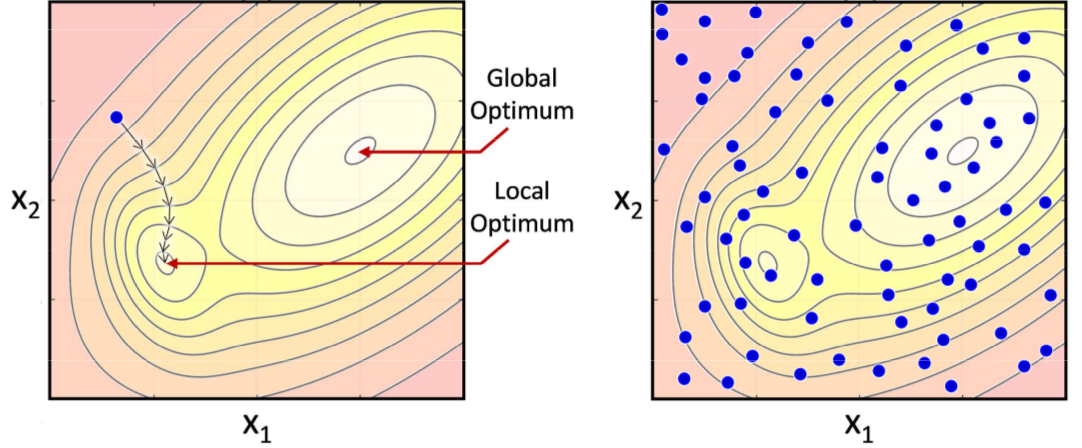
\includegraphics[width=0.6\textwidth]{exploration_2.png}
%\caption{Clasificación de las Meta-heurísticas más populares\footcite{beheshti2013review}.}
\label{fig:clasificacion}
\end{figure}

\end{frame}

\begin{frame}{¿Cómo tratar la convergencia?}
\begin{itemize}
\justifying
    \item Una grado de exploración elevado puede causar una falta de intensificación en las regiones más prometedoras (\textbf{alta diversidad}).
    \item Por otra parte, una intensificación elevada provoca una pérdida de \textbf{diversidad} en la población.
    \item ¿Cómo fomentar este balanceo en una meta-heurística poblacional? (línea de investigación activa).
\end{itemize}
\end{frame}

\begin{frame}{¿Cómo tratar la convergencia?}
\begin{itemize}
\justifying
    \item Algunas técnicas controlan de manera directa o indirecta la cantidad de diversidad mantenida por el algoritmo\footcite{Crepinsek:13}.
    \item Éstas técnicas son identificadas de forma general como enfoques uni-proceso y multi-proceso.
    \item Una taxonomía ampliamente utilizada de las estrategias para promover la diveridad son:
    \begin{itemize}
        \item Enfoques basados en la selección \footcite{eiben2003introduction}.
        \item Enfoques basados en población\footcite{alba2005parallel}.
        \item Enfoques basados en la cruza y/o la mutación\footcite{yu2014differential}.
    \end{itemize}
\end{itemize}
\end{frame}


\begin{frame}{Esquemas de reemplazamiento basados en diversidad}
\begin{itemize}
    \item Los esquemas de reemplazamiento se utilizan para diversificar a los individuos sobrevivientes, de forma que los operadores de reproducción puedan generar nuevas soluciones en diferentes regiones \footcite{eiben1998evolutionary}.
    \item Existen varias estrategias de reemplazo para forzar la diversidad en la población, algúnas populares son:
    \begin{itemize}
    \scriptsize
       \item \textit{Restricted Tournament Selection} - RTS (\citeyear{harik1995finding}) por \citeauthor{harik1995finding}.
       \item \textit{Contribution of Diversity and Replacement of the Worst} - CD/RW (\citeyear{lozano2008replacement}) por \citeauthor{lozano2008replacement}.
       \item \textit{Hybrid Genetic Search with Adaptive Diversity Control} - HGSADC (\citeyear{vidal2013hybrid}) por \citeauthor{vidal2013hybrid}.
       \item \textit{Multi-dynamic} (\citeyear{segura2016novel}) por \citeauthor{segura2016novel}. 
       \item \textit{Best-Non Penalized} (\citeyear{romero2018memetic}) por \citeauthor{romero2018memetic}.
    \end{itemize}
\end{itemize}
\end{frame}

\section{Conceptos}

\begin{frame}{Definición de un problema mono-objetivo}
    \begin{itemize}
\justifying
\item Un problema de optimización mono-objetivo puede ser definido de la siguiente forma\footcite{nocedal2006numerical}:
%
\end{itemize}
\begin{equation}
\scriptsize
\begin{split}
Minimizar/Maximizar \quad &f(x)  \\
sujeto\quad a \quad  &g_j(x) \geq 0 \quad j = 1,2, ... J\\
&h_k(x) = 0, \quad k=1,2, ..., K\\
&x_i^{(L)} \leq x_i \leq x_i^{(U)} \quad i = 1,2, ..., n 
\end{split}
\label{eqn:MOOP}
\end{equation}
donde $x_i^{(L)}, x_i^{(U)}$ son el límite inferior y superior de la $i$-ésima variable, $g_j(x)$ y $h_k(x)$ son restricciones de desigualdad e igualdad respectivamente.
%
%\begin{itemize}
%    \item Si el problema tiene dominio continuo $x \in \Re^n$.
%\end{itemize}
\end{frame}



\begin{frame}{Definición de un problema multi-objetivo}
\begin{itemize}
    \item Un problema de optimización multi-objetivo tiene un número de funciones objetivo en conflicto las cuales se deben minimizar o maximizar.
    \item Similarmente a un problema de optimización mono-objetivo, un problema multi-objetivo tiene un número de restricciones que cualquier solución factible debería satisfacer.
\end{itemize}

La forma general de un problema multi-objetivo se puede definir de la siguiente forma\footcite{Joel:Kalyanmoy}:
\begin{equation}
\scriptsize
\begin{split}
Minimizar/Maximizar \quad &f_m(x), \quad m=1,2,...,M  \\
sujeto\quad a \quad  &g_j(x) \geq 0 \quad j = 1,2, ... J\\
&h_k(x) = 0, \quad k=1,2, ..., K\\
&x_i^{(L)} \leq x_i \leq x_i^{(U)} \quad i = 1,2, ..., n 
\end{split}
\label{eqn:MOOP}
\end{equation}
%donde $x_i^{(L)}, x_i^{(U)}$ son el límite inferior y superior de la $i$-ésima variable respectivamente.
\end{frame}



\begin{frame}{Definición de dominancia}
\justifying
\begin{itemize}
\justifying
    \item A diferencia del caso mono-objetivo, en el ámbito multi-objetivo no es posible comparar de forma directa dos soluciones $x, y \in \Omega$.
    \item Una alternativa para comparar soluciones es considerando la relación de dominancia.
\end{itemize}

\begin{mydef}{Dominancia}{theoexample}
\scriptsize
Se dice que una solución $x$ domina a otra solución $y$ ($x \prec y$), si se cumplen las siguientes dos condiciones:
    \begin{itemize}
        \item La solución $x$ no es peor que la solución $y$ en ninguno de los objetivos.\\
$\forall m \in \{ 1, 2, ..., M \}: f_m(x) \leq f_m(y)$
\justifying
        \item La solución $x$ es estrictamente mejor que la solución $y$ en al menos un objetivo.\\
$\exists m \in \{ 1, 2, ..., M \}: f_m(x) < f_m(y)$
    \end{itemize}
\end{mydef}
\end{frame}

\begin{frame}{Dominancia}
\begin{figure}[H]
\centering
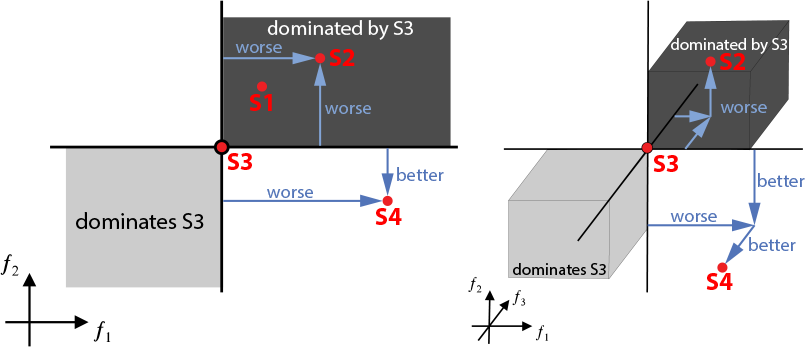
\includegraphics[width=0.9\textwidth]{dominance_scheme.png}
\caption{\scriptsize Esquema de dominancia en dos y tres objetivos respectivamente\footcite{WinNT}.}
\end{figure}
\end{frame}

\begin{frame}{Conceptos multi-objetivo}

\begin{mydef}{ \scriptsize Conjunto no dominado}{theoexample}
\scriptsize
    \item Es la colección de todas la soluciones incomparables y no dominadas relacionadas al conjunto $S \subseteq \Omega$ .
    \begin{equation*}
        NDS(S) = \{ s \in S: \nexists s\prime \in S, s\prime \prec s \}
    \end{equation*}
\end{mydef}

\begin{mydef}{\scriptsize Conjunto Óptimo de Pareto}{theoexample}
\scriptsize
%\begin{itemize}
%    \item 
Es un conjunto de vectores de decisión óptimos no dominados en $\Omega$.
       \begin{equation*}
        POS = \{ x^* \in \Omega : \nexists x \in \Omega \subset \Re^n, x \prec x^*  \}
    \end{equation*}
%\end{itemize}{}
\end{mydef}

\begin{mydef}{\scriptsize Frente de Pareto}{theoexample}
\scriptsize
%\begin{itemize}
    %\item 
    La imágen del conjunto óptimo de Pareto es el frente de Pareto óptimo. 
        \begin{equation*}
             POF = \{ f(x^*) \in Z \subset \Re^m: x^* \in POS \} 
        \end{equation*}
%\end{itemize}{}
\end{mydef}

%\begin{figure}[H]
%\centering
%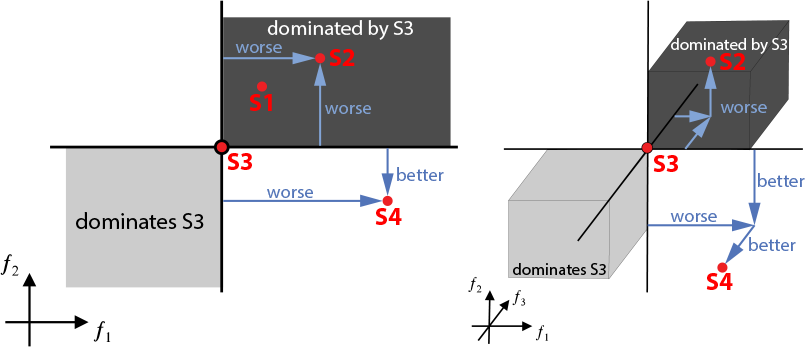
\includegraphics[width=0.8\textwidth]{dominance_scheme.png}
%\caption{\scriptsize Definición de dominancia con dos y tres objetivos respectivamente\footcite{WinNT}.}
%\end{figure}
\end{frame}


\begin{frame}{Conceptos multi-objetivo}

\begin{figure}[H]
\centering
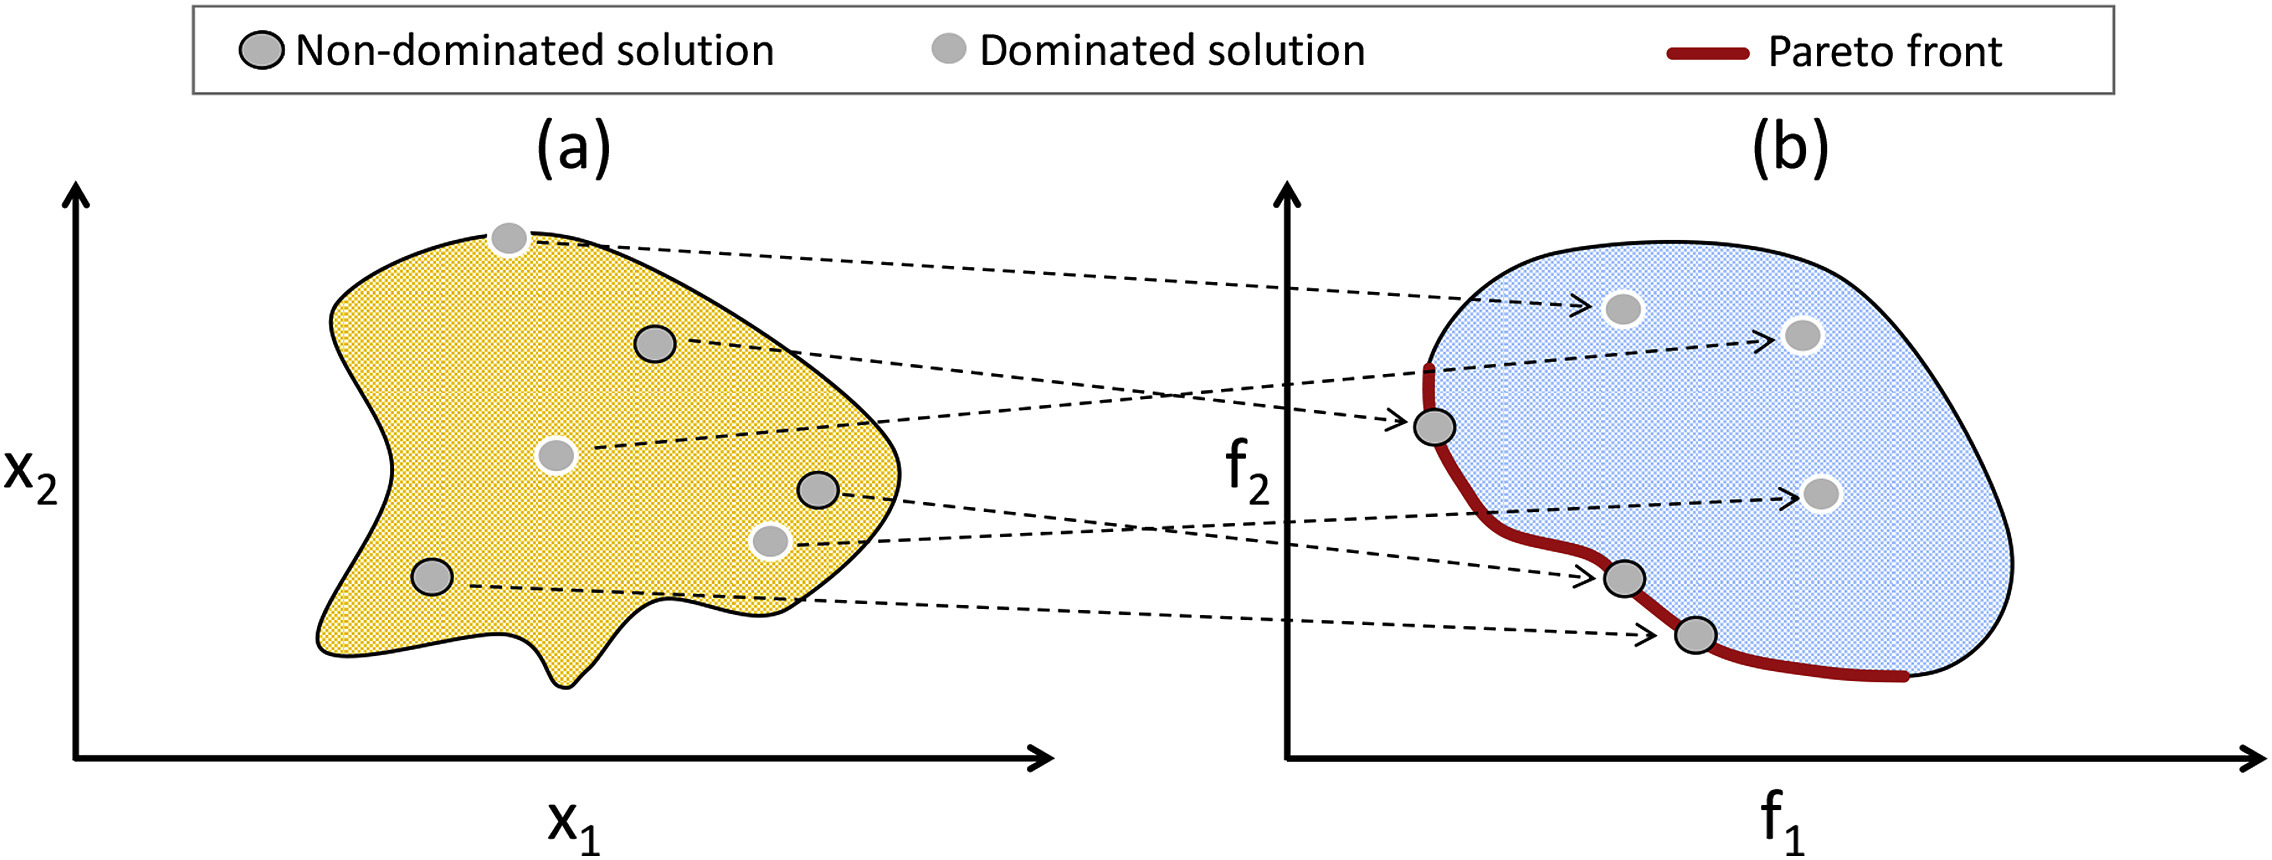
\includegraphics[width=0.9\textwidth]{Mapping.jpg}
\caption{\scriptsize Mapeo del espacio de las variables (a) en el espacio objetivo (b)\footcite{alam2012diversity}.}
\end{figure}
\end{frame}




\section{Paradigmas de algoritmos multi-objetivo}

\begin{frame}{Paradigmas de los algoritmos multi-objetivo}
Una clasificación muy aceptada de los MOEAs es\footcite{trivedi2016survey}:
\begin{itemize}
\justifying
\item \textbf{Basados en dominancia}.
   \begin{itemize}
       \item Utilizan la relación de dominancia de Pareto.
   \end{itemize}
\justifying
\item \textbf{Basados en descomposición}.
\begin{itemize}
       \item Transforman un problema multi-objetivo en un conjunto de problemas de optimización mono-objetivo que son resueltos simultáneamente.
   \end{itemize}
\justifying
\item \textbf{Basados en indicadores}.
    \begin{itemize}
        \item Combinan el grado de convergencia y/o la diversidad en el espacio objetivo con una métrica.
    \end{itemize}
\end{itemize}

\justifying
\scriptsize
Actualmente no existe un algoritmo el cual sea considerado superior, por lo tanto usualmente se selecciona al menos un algoritmo de cada tipo como parte del estado del arte.
\end{frame}





\begin{frame}{Algoritmos basados en dominancia}
Algunos de los clásicos algoritmos multi-objetivo basados en dominancia son:
\begin{itemize}
\scriptsize
    %\item  Algoritmo Genético Basado en Ordenación de No Dominados II (\textit{Non-dominated Sorting Genetic Algorithm II} - NSGA-II)\footcite{Joel:NSGAII}.
    \item \citeyear{Joel:MOGA}, \textit{Multi-objective Genetic Algorithm} (MOGA), \\ \citeauthor{Joel:MOGA}.
    \item \citeyear{Joel:NPGA}, \textit{Niche Pareto Genetic Algorithm} (NPGA), \\ \citeauthor{Joel:NPGA}.
    \item \citeyear{zitzler2001spea2}, \textit{Strength Pareto Evolutionary Algorithm} (SPEA2), \\ \citeauthor{zitzler2001spea2}.
    \item \citeyear{Joel:NSGAII},  \textbf{\textit{Non-dominated Sorting Genetic Algorithm II} (NSGA-II)}, \\ \citeauthor{Joel:NSGAII}.
    \item \citeyear{Joel:GDE3}, \textit{Generalized Differential Evolution} (GDE3), \\ \citeauthor{Joel:GDE3}.
\end{itemize}
\end{frame}


\begin{frame}{Non-dominated Sorting Genetic Algorithm II (NSGA-II)}
\begin{itemize}
\scriptsize
\item Es uno de los primeros algoritmos multi-objetivo que introducen elitismo.
\item Realiza una clasificación por frentes de baja complejidad $O(MN^2)$, estrategia ampliamente utilizada en multi-objetivo conocida como \textit{fast-non-dominated-sortig}.
\item Considera un operador de amontonamiento o \textit{crowding}. 
\end{itemize}

\begin{figure}[H]
\centering
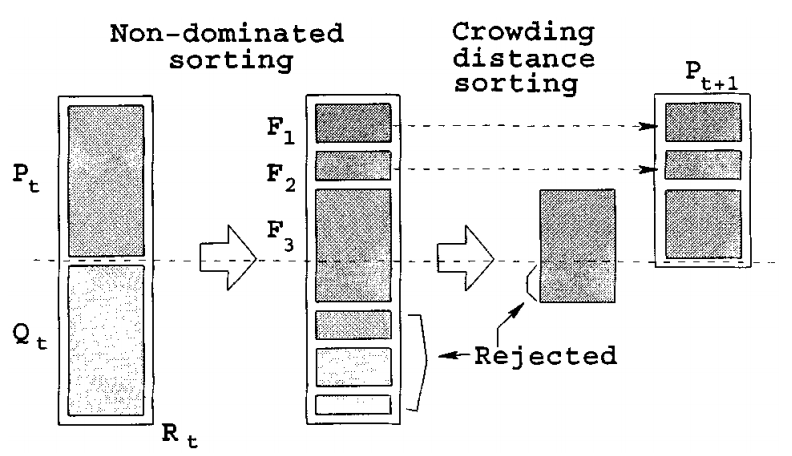
\includegraphics[width=0.7\textwidth]{crowding_nsgaii.png}
\caption{\scriptsize Procedimiento principal del NSGA-II\footcite{Joel:NSGAII}.}
\end{figure}
\end{frame}


\begin{frame}{Non-dominated Sorting Genetic Algorithm II (NSGA-II)}
\begin{itemize}
\scriptsize
\item Es uno de los primeros algoritmos multi-objetivo que introducen elitismo.
\item Realiza una clasificación por frentes de baja complejidad $O(MN^2)$, estrategia ampliamente utilizada en multi-objetivo conocida como \textit{fast-non-dominated-sortig}.
\item Considera un operador de amontonamiento o \textit{crowding}. 
\end{itemize}

\begin{figure}[H]
\centering
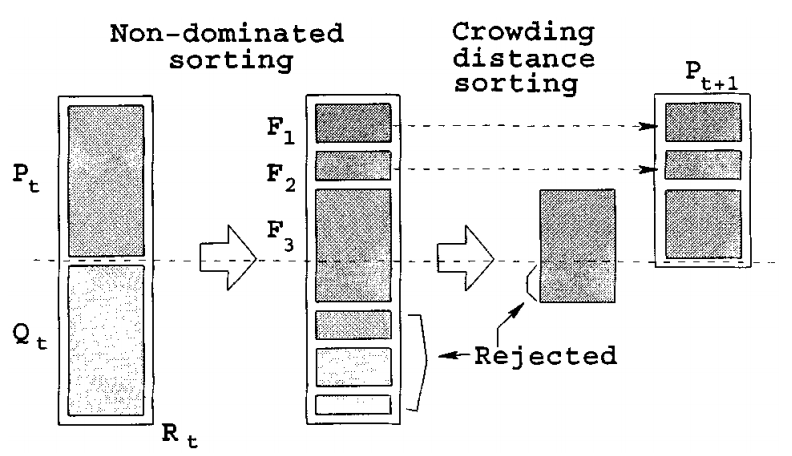
\includegraphics[width=0.7\textwidth]{crowding_nsgaii.png}
\caption{\scriptsize Procedimiento principal del NSGA-II\footcite{Joel:NSGAII}.}
\end{figure}
\end{frame}

 
\begin{frame}{Algoritmos basado en descomposición}
Algunos de los clásicos algoritmos multi-objetivo basados en descomposición son:
\begin{itemize}
     \scriptsize
    \item \citeyear{ishibuchi1998multi}, \textit{Multi-objective Genetic Local Search Algorithm} (MOGLS), \\ \citeauthor{ishibuchi1998multi},
    \item \citeyear{murata2002cellular}, \textit{Cellular Multi-objective Genetic Algorithm} (C-MOGA), \\ \citeauthor{murata2002cellular}, 
    \item \citeyear{Joel:MOEAD}, \textbf{\textit{Multi-objective Evolutionary Algorithm based in Decomposition} (MOEA/D)}, \\ \citeauthor{Joel:MOEAD}.
     \item \citeyear{li2009multiobjective}, \textit{Multi-objective Evolutionary Algorithm based in Decomposition with DE}, (MOEA/D -CEC 2009), \\ \citeauthor{li2009multiobjective}.
    \item \citeyear{Joel:MOEAD_AMS}, \textit{MOEA/D - Adaptive Mating Selection Mechanism} (MOEA/D - AMS) \\ \citeauthor{Joel:MOEAD_AMS}.
    \item \citeyear{zhou2015all}, \textit{MOEA/D - Generalized Resource Allocation} (MOEA/D-GRA) \\ \citeauthor{zhou2015all}.
\end{itemize}
\end{frame}
\begin{frame}{Clasificación por frentes}
    Poner la figura de rankeo.
\end{frame}

\begin{frame}{Multi-objective Evolutionary Algorithm based in Decomposition (MOEA/D)}
\scriptsize
%\item Realiza la descomposición de un problema de optimización multi-objetivo en un conjunto de subproblemas de optimización mono-objetivo de forma simultánea.
MOEA/D\footcite{ishibuchi1998multi}:
\begin{itemize}
\scriptsize
    \item Cada subproblema está definido por un vector de pesos.
    \item Define vecindades de cada subproblema en relación su ubicación en el espacio de los objetivos.
    \item Sólo se hacen emparejamientos y reemplazamientos en los vecindarios.
    \item Considera el operador de cruza SBX y el operador de mutación polinomial.
\end{itemize}
\end{frame}

\begin{frame}{Multi-objective Evolutionary Algorithm based in Decomposition (MOEA/D)}
\begin{itemize}
\scriptsize
\item MOEA/D-DE además considera\footcite{li2009multiobjective}: 
\begin{itemize}
\scriptsize
    \item Reestricciones de emparejamiento y de reemplazamiento.
    \item Para mantener diversidad se considera emparejamiento en toda la población con probabilidad $1 - \delta$ y en el vecindario con probabilidad $\delta$. 
    \item Implementa un mecanismo que administra las evaluaciones de cada subproblema \textit{Dynamical Resource Allocation}.
    \item Utiliza operadores de evolución diferencial y el operador de mutación polinomial.
\end{itemize}
\end{itemize}
\end{frame}



\begin{frame}{Multi-objective Evolutionary Algorithm based in Decomposition (MOEA/D)}

\begin{figure}[H]
\centering
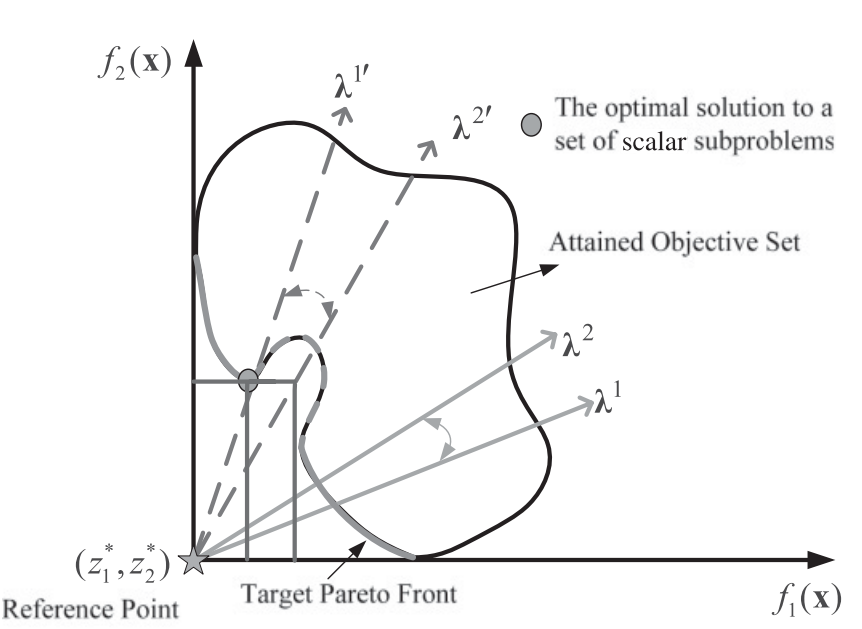
\includegraphics[width=0.6\textwidth]{moead_diagrama.png}
\caption{\scriptsize Vectores de pesos y su punto óptimo con el enfoque de Tchebysheff\footcite{Joel:MOEAD_Adaptative}}
\end{figure}
\end{frame}


\begin{frame}{Funciones de utilidad}
\begin{itemize}
\scriptsize
\item Suma ponderada (\textit{Weighted Sum})
\begin{equation*}
\min_{} g^{ws}(x | \lambda, z^*) = \sum_{i=1}^m \lambda_i f_i(x)     
\end{equation*}
\item Tchebysheff 
\begin{equation*}
    \min_{} g^{te}(x | \lambda, z^*) = \max_{1 \leq i \leq m } \{ \lambda_i | f_i(x) - z_i^* | \}
\end{equation*}{}
\item Función de escalarización alcanzado (\textit{Achieved Scalarized Funcition} - ASF)
\begin{equation*}
    \min_{} g^{te}(x | \lambda, z^*) = \max_{1 \leq i \leq m } \{ \frac{| f_i(x) - z_i^* |}{\lambda_i}\}
\end{equation*}{}
\item Intersección del límite de penalización (\textit{Penalty Boundary Intersection} - PBI)
\begin{equation*}
\begin{split}
    \min g^{bi}(x | \lambda, z^*) &= d_1 + \theta d_2    \\
    sujeto \quad  a \quad d_1 &= \frac{|| (F(x) - z^*)^T \lambda  || }{|| \lambda ||}, \quad d_2 = || F(x) - (z^* + d_1 \lambda )||
\end{split}
\end{equation*}
\end{itemize}
\end{frame}

\begin{frame}{Funciones de utilidad}
\begin{figure}[H]
\begin{tabular}{c c}
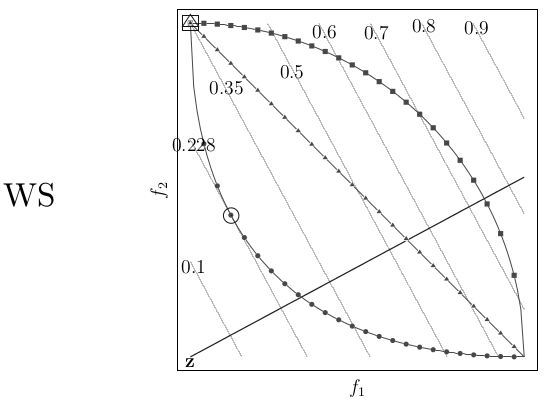
\includegraphics[width=0.4\textwidth]{ws.png}     &  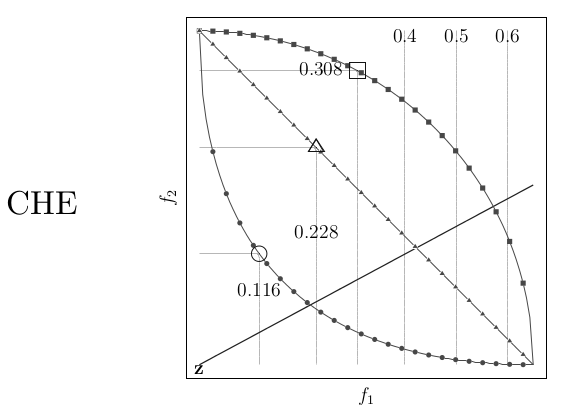
\includegraphics[width=0.4\textwidth]{che.png} \\
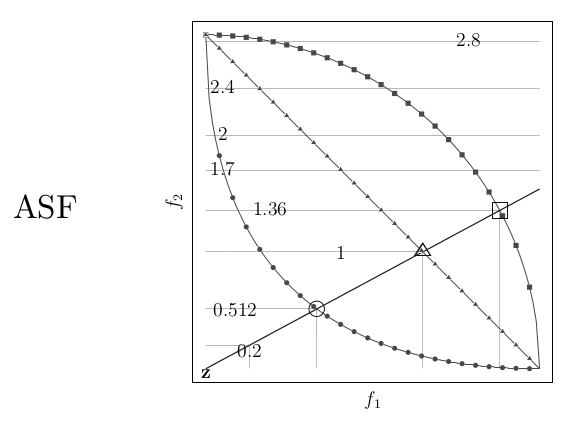
\includegraphics[width=0.4\textwidth]{asf.png}     &  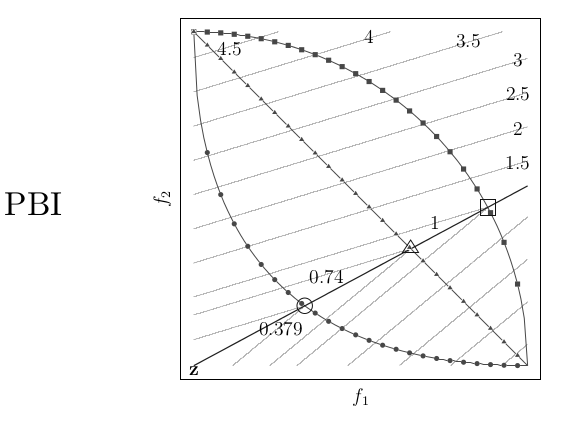
\includegraphics[width=0.4\textwidth]{pbi.png} \\
\end{tabular}
\centering
\caption{\scriptsize Mapa de contorno de las funciones de utilidad.}
\end{figure}
\end{frame}



\begin{frame}{Algoritmos basados en indicadores}
Algunos de los clásicos algoritmos multi-objetivo basados en indicadores son:
\begin{itemize}
\scriptsize
   \item \citeyear{Joel:IBEA}, \textit{Indicator Based-Selection Evolutionary Algorithm } (IBEA), \\ \citeauthor{Joel:IBEA}.
   \item \citeyear{Joel:SMSEMOA}, \textbf{\textit{S-Metric Selection Evolutionary Multi-objective Optimization Algorithm} (SMS-EMOA)}, \\ \citeauthor{Joel:SMSEMOA}.
   \item \citeyear{Joel:FV-MOEA}, \textit{Fast Hypervolume Multi-objective Evolutionary Algorithm} FV-MOEA, \\ \citeauthor{Joel:FV-MOEA}.
   \item \citeyear{Joel:MOMBI-II}, \textit{Many-Objective Metaheuristic Based on $R2$ Indicador} MOMBI-II, \\ \citeauthor{Joel:MOMBI-II}.
\end{itemize}
\end{frame}



\begin{frame}{S-Metric Selection Evolutionary Multi-objective Optimization Algorithm (SMS-EMOA)}
\begin{itemize}
\scriptsize
\item Implementa un operador de selección especial que combina la métrica de hipervolumen con el concepto de dominancia de Pareto.
%
\item Considera un esquema de selección de estado estable (\textit{Steady State}).
\item Una propuesta incorpora la clasificación por frentes y sólo considera el HV cuando la población está compuesta por individuos no dominados.
\end{itemize}
\begin{figure}[H]
\centering
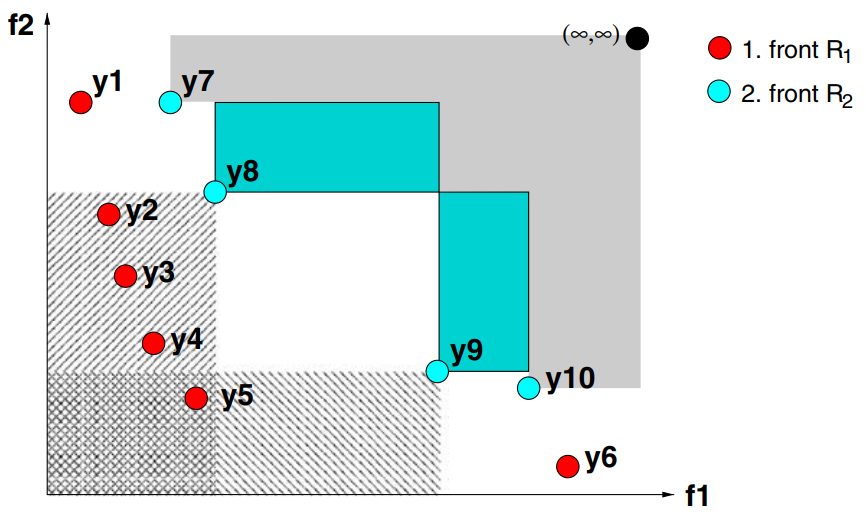
\includegraphics[width=0.6\textwidth]{sms_emoa.png}
\caption{\scriptsize Contribución del HV de cada solución\footcite{Joel:SMSEMOA}.}
\end{figure}
\end{frame}


\begin{frame}{Análisis de los resultados}
Existen distintas herramientas para verificar la calidad de las soluciones de un optimizador, se enlistan las siguientes:
\begin{itemize}
\justifying
\item Métricas de desempeño: son métricas para evaluar la calidad de un conjunto de soluciones no dominadas.
   \begin{itemize}
     \item La Distancia Generacional Invertida (IGD).
     \item La Distancia Generacional Invertida Modificada (IGD+).
     \item El hipervolumen (HV).
   \end{itemize}
\item Análisis estadísticos:
  \begin{itemize}
      \item Pruebas estadísticas.
      \item Tabla general estadística.
  \end{itemize}
  \item Superficies de cubrimiento
\end{itemize}
Poner diagrama de las pruebas estadísticas.
\end{frame}



\begin{frame}{Hipervolumen}
\begin{itemize}
\justifying
\item Es un indicador unario conocido como ``Pareto Compliant''\footcite{zitzler1999evolutionary}.
\item Este indicador determina la porción del espacio objetivo que es dominado por las soluciones de un conjunto $A$, el cual es limitado por un punto de referencia $r \in \Re^n$:
\end{itemize}
\begin{equation}
\scriptsize
    HV(A;r) = \Lambda \left (  \bigcup_{a \in A} \{ x | a \prec x \prec r \} \right )
\end{equation}
donde $\Lambda$ denota la medición de Lebesgue y $r$ debería ser dominado por todos los elementos en $A$.
\begin{figure}[H]
\centering
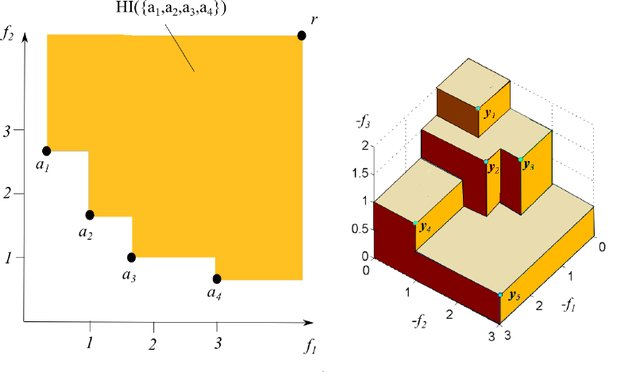
\includegraphics[width=0.55\textwidth]{HV.jpg}
%\caption{\scriptsize Mapeo del espacio de las variables (a) en el espacio objetivo (b)\footcite{alam2012diversity}.}
\end{figure}
\end{frame}
\begin{frame}{Pareto compliant}
    
\end{frame}

\begin{frame}{Distancia generacional}
\begin{itemize}
\justifying
\scriptsize
\item Propociona una noción de distanca entre el frente de Pareto discretizado $R$ y un conjunto aproximado $A$.
\item Consiste en el promedio de las distancias de cada punto de referencia a su solución más cercana $A$:
\end{itemize}
% Please add the following required packages to your document preamble:
% \usepackage{graphicx}
\begin{table}[]
\resizebox{\textwidth}{!}{%
\begin{tabular}{cc}
$IGD(a; R) = \left (  \frac{1}{|R|} \sum_{r \in R} d(r, A)^p \right)^{1/p}$ & $IGD^+(a; R)= \left (  \frac{1}{|R|} \sum_{r \in R} d^+(r, A)^p \right)^{1/p}$ \\ \\
$d = \min_{a \in A} \sqrt{\sum_{i=1}^m (a_i - r_i)^2}$ & $d^+ = \min_{a \in A} \sqrt{\sum_{i=1}^m (max\{ a_i - z_i, 0\})^2}$
\end{tabular}%
}
\end{table}
\begin{figure}[H]
\centering
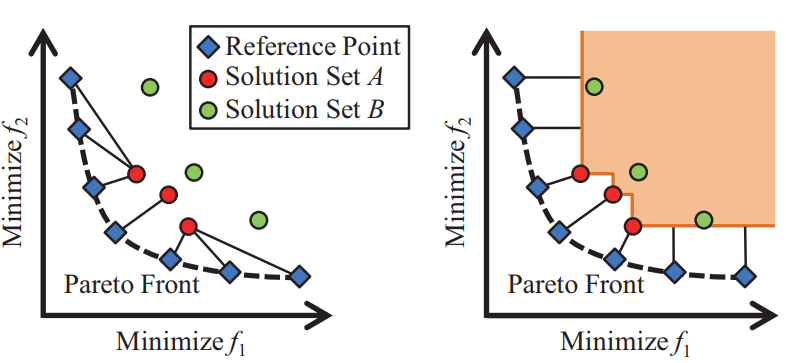
\includegraphics[width=0.55\textwidth]{igd.png}
\caption{\scriptsize Ejemplo de las métricas IGD (izquierda) e IGD+ (derecha).\footcite{ishibuchi2016sensitivity}.}
\end{figure}
\end{frame}


\begin{frame}{Distancia generacional invertida}
\begin{itemize}
\justifying
\scriptsize
\item Propociona una noción de distanca entre el frente de Pareto discretizado $R$ y un conjunto aproximado $A$.
\item Consiste en el promedio de las distancias de cada punto de referencia a su solución más cercana $A$:
\end{itemize}
% Please add the following required packages to your document preamble:
% \usepackage{graphicx}
\begin{table}[]
\resizebox{\textwidth}{!}{%
\begin{tabular}{cc}
$IGD(a; R) = \left (  \frac{1}{|R|} \sum_{r \in R} d(r, A)^p \right)^{1/p}$ & $IGD^+(a; R)= \left (  \frac{1}{|R|} \sum_{r \in R} d^+(r, A)^p \right)^{1/p}$ \\ \\
$d = \min_{a \in A} \sqrt{\sum_{i=1}^m (a_i - r_i)^2}$ & $d^+ = \min_{a \in A} \sqrt{\sum_{i=1}^m (max\{ a_i - z_i, 0\})^2}$
\end{tabular}%
}
\end{table}
\begin{figure}[H]
\centering
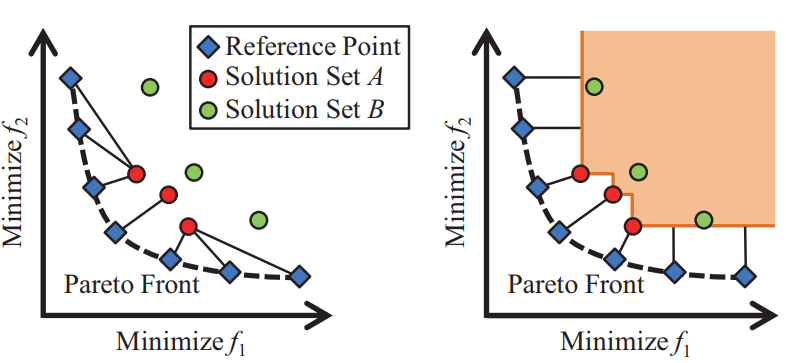
\includegraphics[width=0.55\textwidth]{igd.png}
\caption{\scriptsize Ejemplo de las métricas IGD (izquierda) e IGD+ (derecha).\footcite{ishibuchi2016sensitivity}.}
\end{figure}
\end{frame}



\begin{frame}{Distancia generacional invertida modificada}
\begin{itemize}
\justifying
\scriptsize
\item Propociona una noción de distanca entre el frente de Pareto discretizado $R$ y un conjunto aproximado $A$.
\item Consiste en el promedio de las distancias de cada punto de referencia a su solución más cercana $A$:
\end{itemize}
% Please add the following required packages to your document preamble:
% \usepackage{graphicx}
\begin{table}[]
\resizebox{\textwidth}{!}{%
\begin{tabular}{cc}
$IGD(a; R) = \left (  \frac{1}{|R|} \sum_{r \in R} d(r, A)^p \right)^{1/p}$ & $IGD^+(a; R)= \left (  \frac{1}{|R|} \sum_{r \in R} d^+(r, A)^p \right)^{1/p}$ \\ \\
$d = \min_{a \in A} \sqrt{\sum_{i=1}^m (a_i - r_i)^2}$ & $d^+ = \min_{a \in A} \sqrt{\sum_{i=1}^m (max\{ a_i - z_i, 0\})^2}$
\end{tabular}%
}
\end{table}
\begin{figure}[H]
\centering
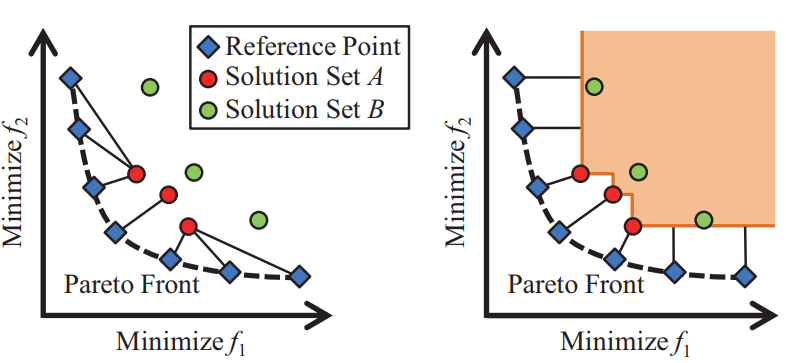
\includegraphics[width=0.55\textwidth]{igd.png}
\caption{\scriptsize Ejemplo de las métricas IGD (izquierda) e IGD+ (derecha).\footcite{ishibuchi2016sensitivity}.}
\end{figure}
\end{frame}


\section{Problemas de prueba}
\begin{frame}{Problemas de prueba en el ámbito multi-objetivo}
\begin{itemize}
   \item ZDT, \citeauthor{Joel:ZDT}, \citeyear{Joel:ZDT}, únicamente de dos objetivos, escalables en las variables.
   \item DTLZ, \citeauthor{Joel:DTLZ_1}, (versión 1 \citeyear{Joel:DTLZ_1}, versión 2 \citeyear{Joel:DTLZ_2}), escalables en los objetivos y las variables.
   \item WFG, \citeauthor{Joel:WFG_Main}, \citeyear{Joel:WFG_Main}, escalables en los objetivos y las variables.
   \item UF, \citeauthor{Joel:CEC2009}, \citeyear{Joel:CEC2009}, únicamente de dos objetivos (UF1-UF7) y tres objetivos (UF8-UF10), escalables en las variables.
\end{itemize}
\end{frame}

\begin{frame}{WFG}
poner imagenes
\begin{itemize}
   \item WFG, \citeauthor{Joel:WFG_Main}, \citeyear{Joel:WFG_Main}, escalables en los objetivos y las variables.
\end{itemize}
\end{frame}


\begin{frame}{UF}
poner imagenes
\begin{itemize}
   \item UF, \citeauthor{Joel:CEC2009}, \citeyear{Joel:CEC2009}, únicamente de dos objetivos (UF1-UF7) y tres objetivos (UF8-UF10), escalables en las variables.
\end{itemize}
\end{frame}



\begin{frame}{Superficie de cubrimiento}
Superficie de cubrimiento.
\end{frame}

\section{Convergencia en algoritmos evolutivos}

\begin{frame}{Componentes de un algoritmo evolutivo}
Poner los componentes de un algoritmo evolutivo    
\end{frame}

\begin{frame}{Esquema Best No Penalized}
Poner esquema del BNP
\end{frame}


\begin{frame}{Análisis preliminar}
\begin{itemize}
\scriptsize
\justifying
\item Se utilizan los problemas WFG \textit{The Walking Fish Group}.
\justifying
\item Estos problemas dividen a las variables de desición en dos tipos: las variables de distancia y las variables de posición.
\end{itemize}
\begin{figure}
\centering
\begin{tabular}{c}
 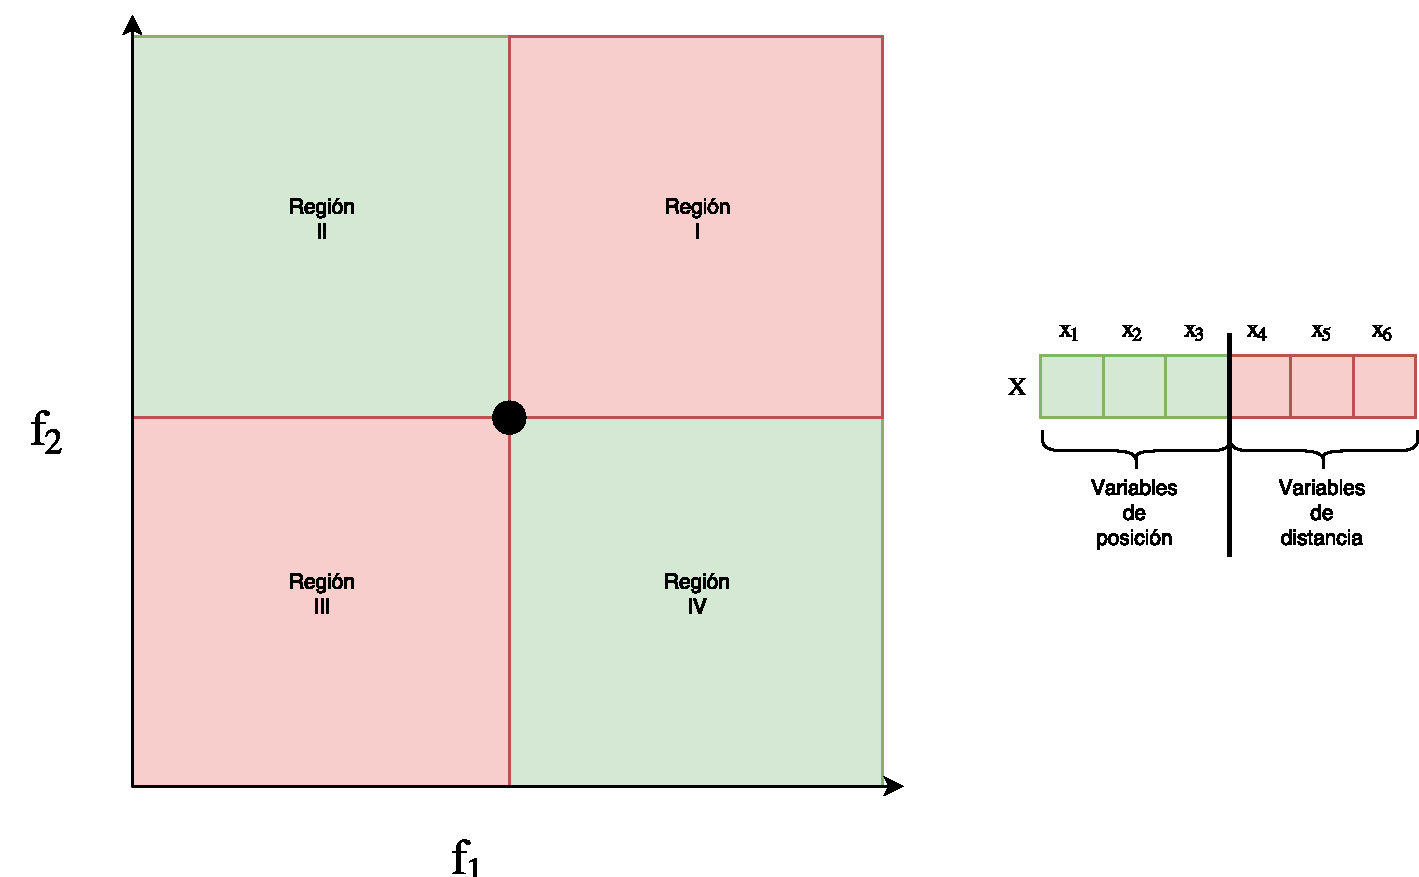
\includegraphics[width=0.9\textwidth]{Parametros_Posicion_Distancia.pdf}   \\
\end{tabular}
\caption{Variables de posición y distancia de los problemas WFG.}
\end{figure}
\end{frame}




\begin{frame}{Análisis preliminar}
\begin{itemize}
\justifying
\item Se eligen los algoritmos NSGA-II, GDE3, MOEA/D y MOMBI-II, siendo basados en dominancia los dos primeros, y basados en descomposición e indicadores los dos últimos.
\justifying
\item Se selecciona el problema de prueba WFG1 que aunque posee una definición simple, muchos MOEAs tienen dificultades de resolverlo.
\justifying
\item Específicamente, la instancia WFG1 es un problema uni-modal y separable.

\end{itemize}
\end{frame}

\begin{frame}{Análisis preliminar}
\begin{itemize}
\justifying
\item La región óptima para el WFG1 esta indicada en la ecuación (\ref{optimo}), donde $k$ es el número de variables de posición y $k+1$ a $n$ son las variables de distancia.
\end{itemize}

\begin{equation} \label{optimo}
	x_{i=k+1:n} = 2i \times 0.35
\end{equation}

\end{frame}

\begin{frame}{Análisis preliminar}
\begin{itemize}
\justifying
\item Se realizaron $35$ ejecuciones con un criterio de paro de $50'000$ generaciones y el tamaño de población de $250$.
\justifying
\item Particularmente, el análisis de diversidad es considerando en las variables de distancia.
\end{itemize} 
\end{frame}




\begin{frame}{Análisis preliminar}
\begin{itemize}
\justifying
\item Se calcula la distancia promedio entre los individuos (ADI \textit{Average Distance to all Individuals}).
\justifying
\item En relativamente pocas generaciones (aproximadamente $5'000$), las variables de distancia convergen en todos los métodos.
\justifying
\item En algunas generaciones se recupera la diversidad por el efecto del operador de mutación polinomial.
\end{itemize}
\begin{figure}
\centering
\begin{tabular}{cc}
 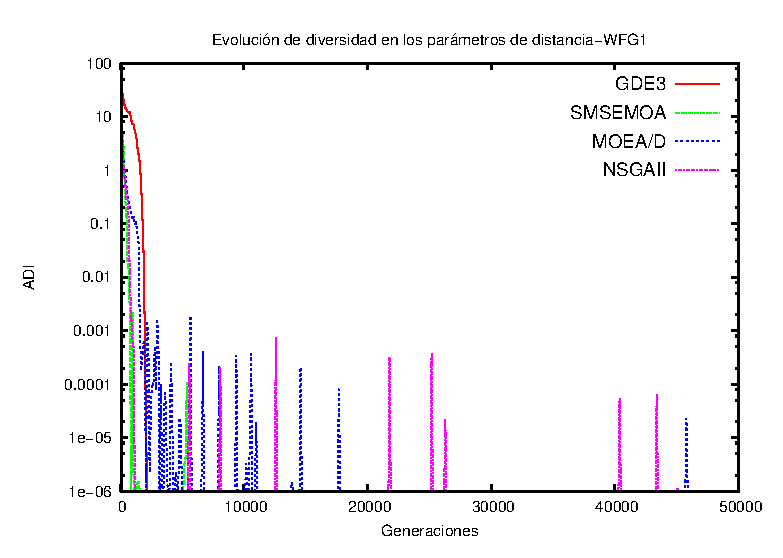
\includegraphics[width=0.5\textwidth]{Average_DistanceParamsStateArt.eps} 
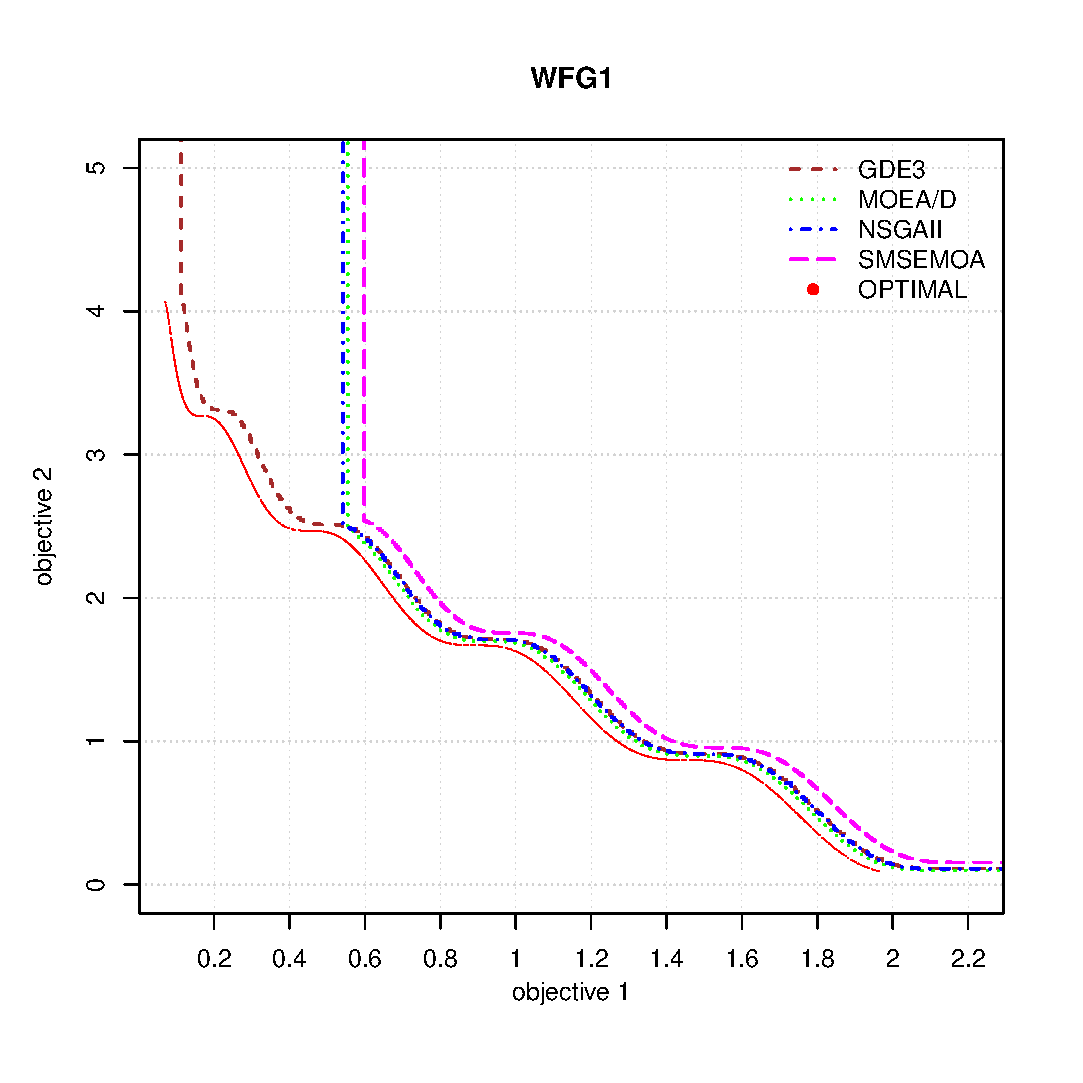
\includegraphics[width=0.35\textwidth]{WFG1_analisis.eps} %\\
\end{tabular}
\caption{Evolución de la diversidad y superficie de alcance al 50\%.}
\label{fig:DiversityProposal}
\end{figure}
\end{frame}


\begin{frame}{Hipótesis}
poner hipótesis....
\end{frame}


\section{Algoritmo de diversidad basado en dominancia}

\begin{frame}{Procedimiento principal del VSD-MOEA}
\begin{itemize}
\justifying
\item Se propone al VSD-MOEA (\textit{Variable Space Diversity - Multi-objective Evolutionary Algorithm}).
\justifying
\item Se utiliza el esquema usual de un Algoritmo Evolutivo (EA - \textit{Evolutionary Algorithm}).
\justifying
\item Se establece una fase especial de reemplazo, donde se define un procedimiento para administrar de forma explícita la diversidad.
\end{itemize}
\begin{figure}
\centering
\begin{tabular}{c}
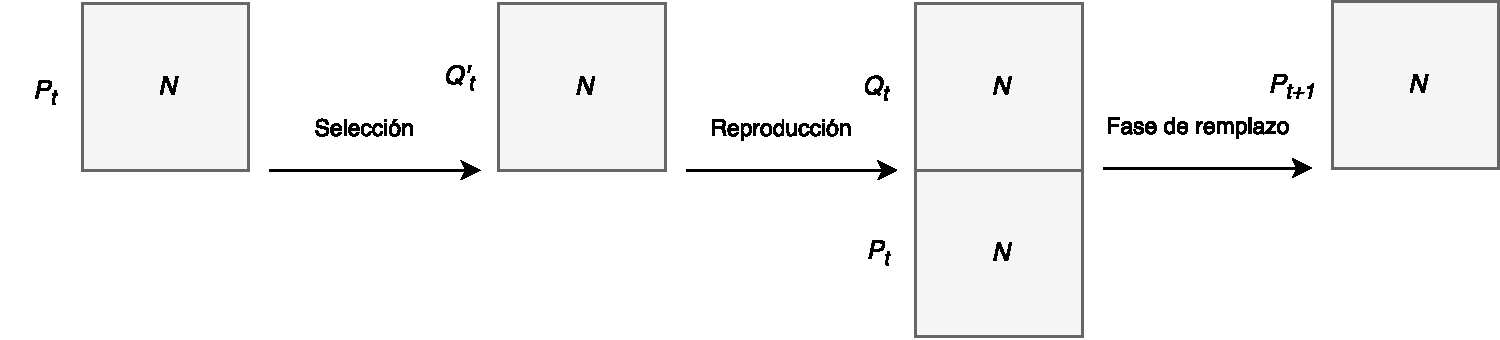
\includegraphics[width=0.9\textwidth]{Evolution_Process.pdf}
\end{tabular}
\caption{Proceso realizado en cada generación.}
\label{fig:DiversityProposal}
\end{figure}
\end{frame}


\begin{frame}{Fase de reemplazo}
\begin{itemize}
\justifying
\item La fase de reemplazo considera un método de penalización.
\justifying
\item El radio de la hiperesfera es decrementado conforme transcurre la ejecución.
\end{itemize}
\begin{figure}
\centering
\begin{tabular}{cc}
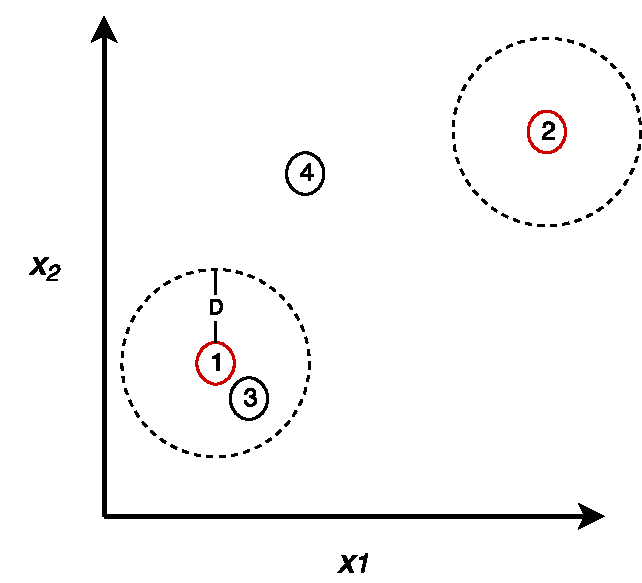
\includegraphics[width=0.35\textwidth]{Metodo_Penalizacion.pdf} \quad \quad \quad
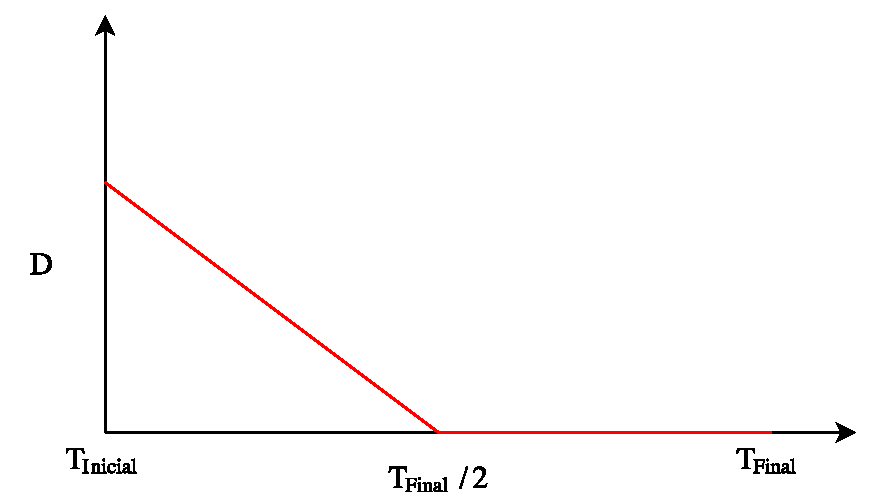
\includegraphics[width=0.6\textwidth]{Modelo.pdf}
\end{tabular}
\label{fig:DiversityProposal}
\end{figure}
\end{frame}



\begin{frame}{Esquema general de la propuesta basada en dominancia}
    \begin{algorithm}[H]
    \begin{scriptsize}
%\algsetup{linenosize=\tiny}
	\caption{Main procedure of VSD-MOEA} 
	\begin{small}
\begin{algorithmic}[1]
 	\STATE \textbf{Initialization}: Generate an initial population $P_0$ with $N$ individuals.
	\STATE \textbf{Evaluation}: Evaluate all individuals in the population.
	\STATE Assign $t=0$
	\WHILE{ (not stopping criterion)  }
	   \STATE \textbf{Mating selection}: Fill the mating pool by performing binary tournament selection on $P_t$, 
		 based on the non-dominated ranks (ties are broken randomly).
	   \STATE \textbf{Variation}: Apply SBX crossover and Polynomial mutation to the mating pool to create a child population $Q_t$.
		 \STATE \textbf{Evaluation}: Evaluate all individuals in $Q_t$.
	   \STATE \textbf{Survivor selecction}: Generate $P_{t+1}$ by applying the replacement scheme 
		 described in Algorithm \ref{alg:Replacement_Phase}, using $P_t$ and $Q_t$ as input.
	   \STATE $t=t+1$
	\ENDWHILE
	\end{algorithmic}
	\end{small}
\label{alg:vsd-moea}
\end{scriptsize}
\end{algorithm}
\end{frame}

\begin{frame}{Fase de reemplazo}
Principalmente, la fase de reemplazo se basa en un método de penalización que implementa la métrica de mejoría. \\
($D^b(p_i, r_i) =& \sum_{i \in M} max\{0, p_i - r_i\}^2$).
\begin{figure}[t]
\centering




\tikzset{every picture/.style={line width=0.75pt}} %set default line width to 0.75pt        

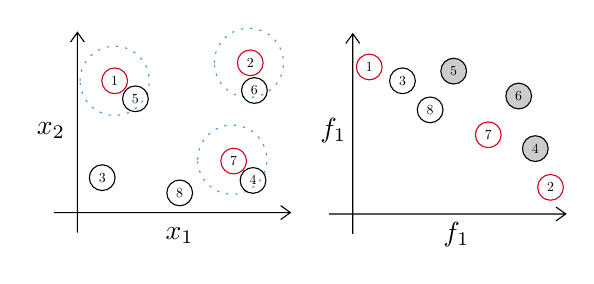
\begin{tikzpicture}[x=0.5pt,y=0.5pt,yscale=-1,xscale=1]
%uncomment if require: \path (0,300); %set diagram left start at 0, and has height of 300

%Shape: Circle [id:dp5136866411017809] 
\draw  [color={rgb, 255:red, 74; green, 144; blue, 226 }  ,draw opacity=1 ][dash pattern={on 0.84pt off 2.51pt}] (69,105) .. controls (69,91.19) and (80.19,80) .. (94,80) .. controls (107.81,80) and (119,91.19) .. (119,105) .. controls (119,118.81) and (107.81,130) .. (94,130) .. controls (80.19,130) and (69,118.81) .. (69,105) -- cycle ;
%Shape: Circle [id:dp3061612047883613] 
\draw  [color={rgb, 255:red, 74; green, 144; blue, 226 }  ,draw opacity=1 ][dash pattern={on 0.84pt off 2.51pt}] (166,92) .. controls (166,78.19) and (177.19,67) .. (191,67) .. controls (204.81,67) and (216,78.19) .. (216,92) .. controls (216,105.81) and (204.81,117) .. (191,117) .. controls (177.19,117) and (166,105.81) .. (166,92) -- cycle ;
%Shape: Axis 2D [id:dp3645341276574614] 
\draw  (50,200.22) -- (221,200.22)(67.1,70) -- (67.1,214.69) (214,195.22) -- (221,200.22) -- (214,205.22) (62.1,77) -- (67.1,70) -- (72.1,77)  ;
%Shape: Circle [id:dp595877391054507] 
\draw  [color={rgb, 255:red, 74; green, 144; blue, 226 }  ,draw opacity=1 ][dash pattern={on 0.84pt off 2.51pt}] (154,162) .. controls (154,148.19) and (165.19,137) .. (179,137) .. controls (192.81,137) and (204,148.19) .. (204,162) .. controls (204,175.81) and (192.81,187) .. (179,187) .. controls (165.19,187) and (154,175.81) .. (154,162) -- cycle ;
%Shape: Axis 2D [id:dp14963900792703488] 
\draw  (249,201.22) -- (420,201.22)(266.1,71) -- (266.1,215.69) (413,196.22) -- (420,201.22) -- (413,206.22) (261.1,78) -- (266.1,71) -- (271.1,78)  ;

% Text Node
\draw  [color={rgb, 255:red, 208; green, 2; blue, 27 }  ,draw opacity=1 ]  (94, 105) circle [x radius= 9.3, y radius= 9.3]   ;
\draw (94,105) node [scale=0.5] [align=left] {1};
% Text Node
\draw  [color={rgb, 255:red, 0; green, 0; blue, 0 }  ,draw opacity=1 ]  (109, 118) circle [x radius= 9.3, y radius= 9.3]   ;
\draw (109,118) node [scale=0.5] [align=left] {5};
% Text Node
\draw  [color={rgb, 255:red, 208; green, 2; blue, 27 }  ,draw opacity=1 ]  (192, 92) circle [x radius= 9.3, y radius= 9.3]   ;
\draw (192,92) node [scale=0.5] [align=left] {2};
% Text Node
\draw    (195, 112) circle [x radius= 9.3, y radius= 9.3]   ;
\draw (195,112) node [scale=0.5] [align=left] {6};
% Text Node
\draw  [color={rgb, 255:red, 208; green, 2; blue, 27 }  ,draw opacity=1 ]  (180, 163) circle [x radius= 9.3, y radius= 9.3]   ;
\draw (180,163) node [scale=0.5] [align=left] {7};
% Text Node
\draw    (194, 177) circle [x radius= 9.3, y radius= 9.3]   ;
\draw (194,177) node [scale=0.5] [align=left] {4};
% Text Node
\draw    (141, 186) circle [x radius= 9.3, y radius= 9.3]   ;
\draw (141,186) node [scale=0.5] [align=left] {8};
% Text Node
\draw    (85, 175) circle [x radius= 9.3, y radius= 9.3]   ;
\draw (85,175) node [scale=0.5] [align=left] {3};
% Text Node
\draw  [color={rgb, 255:red, 208; green, 2; blue, 27 }  ,draw opacity=1 ]  (278, 95) circle [x radius= 9.3, y radius= 9.3]   ;
\draw (278,95) node [scale=0.5] [align=left] {1};
% Text Node
\draw  [color={rgb, 255:red, 0; green, 0; blue, 0 }  ,draw opacity=1 ][fill={rgb, 255:red, 0; green, 0; blue, 0 }  ,fill opacity=0.2 ]  (339, 98) circle [x radius= 9.3, y radius= 9.3]   ;
\draw (339,98) node [scale=0.5] [align=left] {5};
% Text Node
\draw  [color={rgb, 255:red, 208; green, 2; blue, 27 }  ,draw opacity=1 ]  (409, 182) circle [x radius= 9.3, y radius= 9.3]   ;
\draw (409,182) node [scale=0.5] [align=left] {2};
% Text Node
\draw  [fill={rgb, 255:red, 0; green, 0; blue, 0 }  ,fill opacity=0.2 ]  (386, 116) circle [x radius= 9.3, y radius= 9.3]   ;
\draw (386,116) node [scale=0.5] [align=left] {6};
% Text Node
\draw  [color={rgb, 255:red, 208; green, 2; blue, 27 }  ,draw opacity=1 ]  (364, 144) circle [x radius= 9.3, y radius= 9.3]   ;
\draw (364,144) node [scale=0.5] [align=left] {7};
% Text Node
\draw  [fill={rgb, 255:red, 0; green, 0; blue, 0 }  ,fill opacity=0.2 ]  (398, 154) circle [x radius= 9.3, y radius= 9.3]   ;
\draw (398,154) node [scale=0.5] [align=left] {4};
% Text Node
\draw    (322, 126) circle [x radius= 9.3, y radius= 9.3]   ;
\draw (322,126) node [scale=0.5] [align=left] {8};
% Text Node
\draw    (302, 105) circle [x radius= 9.3, y radius= 9.3]   ;
\draw (302,105) node [scale=0.5] [align=left] {3};
% Text Node
\draw (141,217) node   {$x_{1}$};
% Text Node
\draw (48,141) node   {$x_{2}$};
% Text Node
\draw (341,216) node   {$f_{1}$};
% Text Node
\draw (252,141) node   {$f_{1}$};


\end{tikzpicture}


%\includegraphics[width=0.45\textwidth]{Images/Fase_Remplazo_2.eps}
\caption{Método de penalización de la fase de reemplazo.} \label{fig:Hypersphere}
\end{figure}
\end{frame}

\begin{frame}{Procedimiento de selección}
El estimador de densidad en el espacio objetivo considera el indicador ASF y la distancia de mejoría.
\begin{equation}\label{eqn:extremes}
\scriptsize
AWF_k (\vec{x}) = f_k(\vec{x}) + 10^{-4} \times  \sum_{j=1}^M f_j( \vec{x} )
\end{equation}

%\begin{itemize}
%\justifying
%\item Seleccionar al individuo con la mayor distancia al vecino de re\-fe\-ren\-cia más cercano, puede causar selecciones no deseables, como se puede observar en la siguiente imágen.
%\end{itemize}
\begin{figure}[H]
\centering
\scriptsize
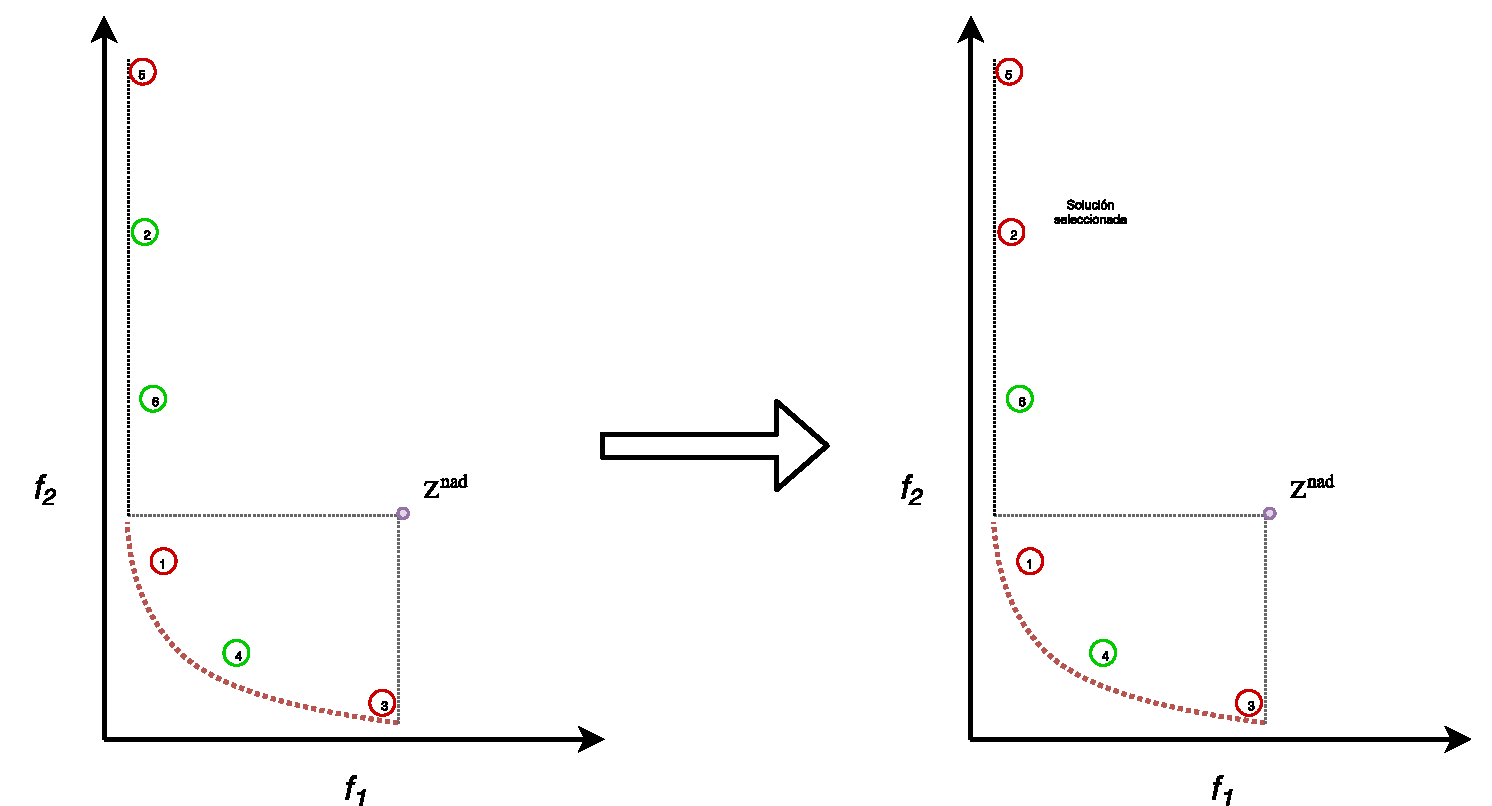
\includegraphics[scale=0.35]
{Atipico.pdf}
%\caption{ Análisis del procedimiento de selección propuesto, las soluciones de referencia están representadas con bordes de color rojo, las soluciones candidatas con bordes de color verde, el frente de Pareto está representado por una línea roja punteada.}
\label{fig:Atipico}
\end{figure}
\end{frame}


\begin{frame}{Fase de reemplazo}
  \begin{algorithm}[H]
  \begin{scriptsize}
%\algsetup{linenosize=\tiny}
	\caption{Replacement Phase of VSD-MOEA} 

\begin{algorithmic}[1]
\STATE Input: $P_t$ (Population of current generation), $Q_t$ (Offspring of current Generation)
    	\STATE Output: $P_{t+1}$ 
        \STATE $R_t = P_t \cup Q_t$ \label{alg:1}
        \STATE $P_{t+1} = \emptyset$ \label{alg:2}
        \STATE $Penalized = \emptyset$ \label{alg:3}
				\STATE $D_t = D_I - D_I * \frac{G_{Elapsed}}{0.9*G_{End}}$ \label{alg:4}
%				\FOR{$k \in {1...M}$}\label{alg:5}
%					\STATE Move to $P_{t+1}$ the individual that optimize $AWF_k$ (Eq.~\ref{eqn:extremes}) \label{alg:5b}
%				\ENDFOR
        \WHILE{ $|P_{t+1}|$ $\leq$ N } \label{alg:6}
					\STATE Compute $DCS$ of individuals in $R_t$ with $P_{t+1}$ used as reference set \label{alg:7}
					\STATE Move to $Penalized$ the individuals in $R_t$ with $DCS < D_t$  \label{alg:8}
        	\IF{$R_t$ is empty} \label{alg:9}
						\STATE Compute $DCS$ of individuals in $Penalized$ with $P_{t+1}$ used as reference set \label{alg:10}
						\STATE Move to $R_t$ the individual in $Penalized$ with largest $DCS$ \label{alg:11}
        	\ENDIF
					\STATE Identify the first front ($F$) in $R_t \cup P_{t+1}$ with an individual $I \in R_t$ \label{alg:12}
					\STATE Use the novel density estimator  to select a new survivor 
					from $F$ and move it to $P_{t+1}$\label{alg:13}
        \ENDWHILE
    	\RETURN $P_{t+1}$ \label{alg:14}
	\end{algorithmic}

\label{alg:Replacement_Phase}
\end{scriptsize}
\end{algorithm}
\end{frame}


\begin{frame}{Comparación del estado-del-arte con ejecuciones a largo plazo}

\end{frame}


\begin{frame}{Pruebas estadísticas}
\end{frame}

\begin{frame}{Estadísticas}

\end{frame}


\begin{frame}{Superficies de cubrimiento}
Poner superficie de diferencias.
\end{frame}

\begin{frame}{Análisis de escalabilidad en el espacio de las variables}
\end{frame}

\begin{frame}{Análisis de rendimiento en función al criterio de paro}
\end{frame}


\begin{frame}{Análisis del umbral de diversidad inicial}
\end{frame}


\begin{frame}{Trabajo en progreso}
\begin{itemize}
    \item Algoritmo multi-objectivo basado en decomposición (VSD-MOEA).
\end{itemize}
\end{frame}


\begin{frame}{Conclusiones y trabajo futuro}


\end{frame}




\begin{frame}{Acknowledgements}
This work has been supported by the Center for Research in Mathematics.
\end{frame}

\end{document}
